
En este primer apartado nos vamos a concentrar en estudiar al Silicio.

\vspace{0.5cm}

El silicio es un semiconductor del grupo IVA de la tabla periódica con número atómico 14, 
un peso atómico de 28.086 y una densidad de 2.33 Mg / m3. Se derrite a 1410 C. 
La configuración electrónica del átomo de silicio es: (Ne) (3s) 2 (3p) 2, y el radio atómico es 0.132 nm.

\vspace{0.5cm}

El silicio tiene la estructura de cristal cúbico de diamante con un parámetro de red de 0,543 nm. 
La distancia del vecino más cercano es 0.235 nm. 
La estructura de cristal cúbico de diamante tiene una red fcc con una base de dos átomos de silicio.


\begin{figure}[H]
    \centering
    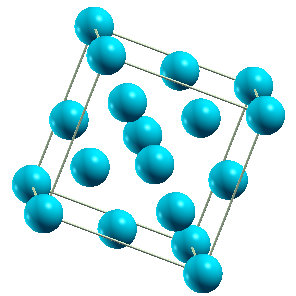
\includegraphics[scale=0.5]{Silicio_scf_init.png}
    \caption{Estructura cristalina del Silicio obtenida del archivo input con Xcrysden}
\end{figure}

\begin{table}[H]
    \begin{center}
        \begin{tabular}{| c | c |}
            \hline
            \multicolumn{2}{ |c| }{Archivo inicial} \\ \hline
            ibrav & 2 \\ \hline
            nat & 2 \\ \hline
            ntype & 1 \\ \hline
            occupations & smearing \\ \hline
            degauss & 0.01 \\ \hline
            Atomic Positions Crystal & Si 0.000 0.000 0.000  \\
                                     & Si 0.250 0.250 0.250 \\  \hline
        \end{tabular}
        \caption{Principales paramétros del silicio}
        \label{tab: Parametros del Silicio}
    \end{center}
\end{table}

A continuación, realizaremos las siguientes optimizaciones:

\begin{itemize}
    \item Optimización Ecutwfc [Silicio]
    \item Optimización Ecutrho [Silicio]
    \item Optimización K-points [Silicio]
    \item Optimización Lattice parameter (parámetro de red) [Silicio]
\end{itemize}

\newpage

\subsection{Optimización Ecutwfc [Silicio] }

En los cálculos de DFT, la elección del Ecutwfc es muy importante y juega un papel decisivo en la 
precisión de los resultados obtenidos. Por esta razón, el primer paso en cualquier trabajo de DFT es 
verificar la convergencia de la propiedad deseada versus esta cantidad.

Buscamos obtener un valor mínimo para el parámetro Ecutwfc donde podamos observar una convergencia en la 
energía del sistema.

\vspace{0.2cm}

Vamos a variar el valor del paramétro Ecutwfc de 20 a 50 en pasos de 5 en 5, así realizaremos un cálculo de
SCF y un ploteo de Ecutwfc contra la energía total de la estructura.

\vspace{0.1cm}

\begin{figure}[H]
    \centering
    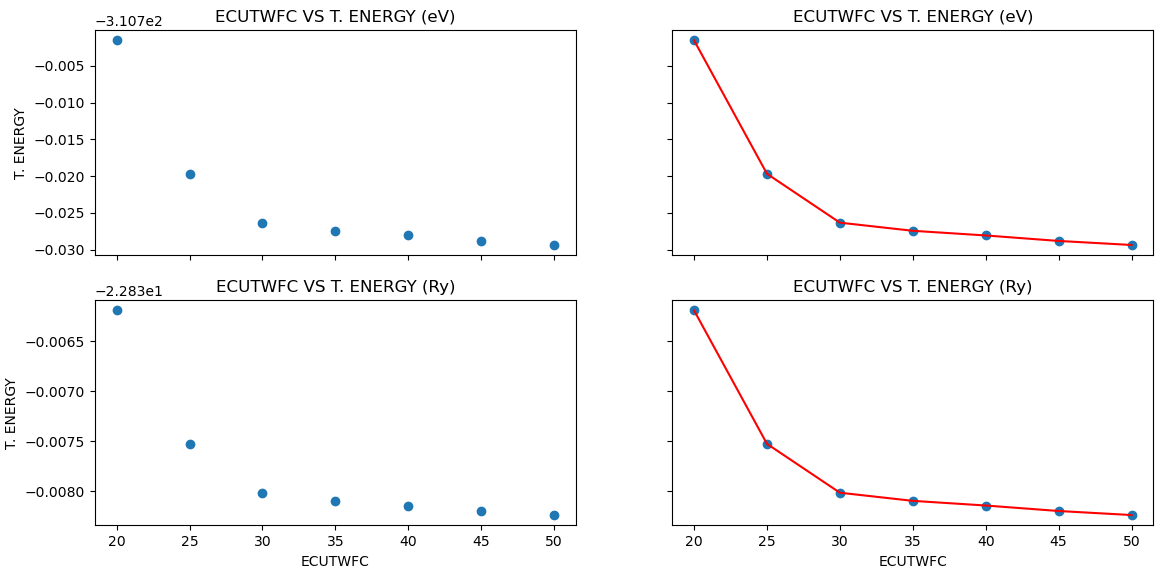
\includegraphics[scale=0.36]{images/ecutwfc_vs_t_energy.png}
    \caption{Gráfica que nos muestra la energía total del sistema contra la variación del parámetro ecutwfc}
\end{figure}


Observación: el valor de la variable dependiente (la energía total) empieza su convergencia cuando 
la variable independiente (ecutwfc) empieza a tomar valores cercanos a 30.

\newpage

\subsection{Optimización Ecutrho [Silicio] }

Ahora vamos a buscar optimizar el valor del paramétro Ecutrho, donde para fines de nuestra actividad 
supondremos que es un múltiplo de el valor que toma Ecutwfc, donde depende de la siguiente forma:

\begin{equation*}
    Ecutrho = k*Ecutwfc
\end{equation*}

Donde $ k \in \mathbb{N}  $

\vspace{0.5cm}

Buscamos obtener un valor mínimo para k de tal manera que podamos observar una convergencia en la 
energía del sistema.

\vspace{0.5cm}

Vamos a variar el valor de k de 1 a 12 en pasos de 1 en 1, así realizaremos un cálculo de
SCF y un ploteo del valor de k contra la energía total de la estructura.

\begin{figure}[H]
    \centering
    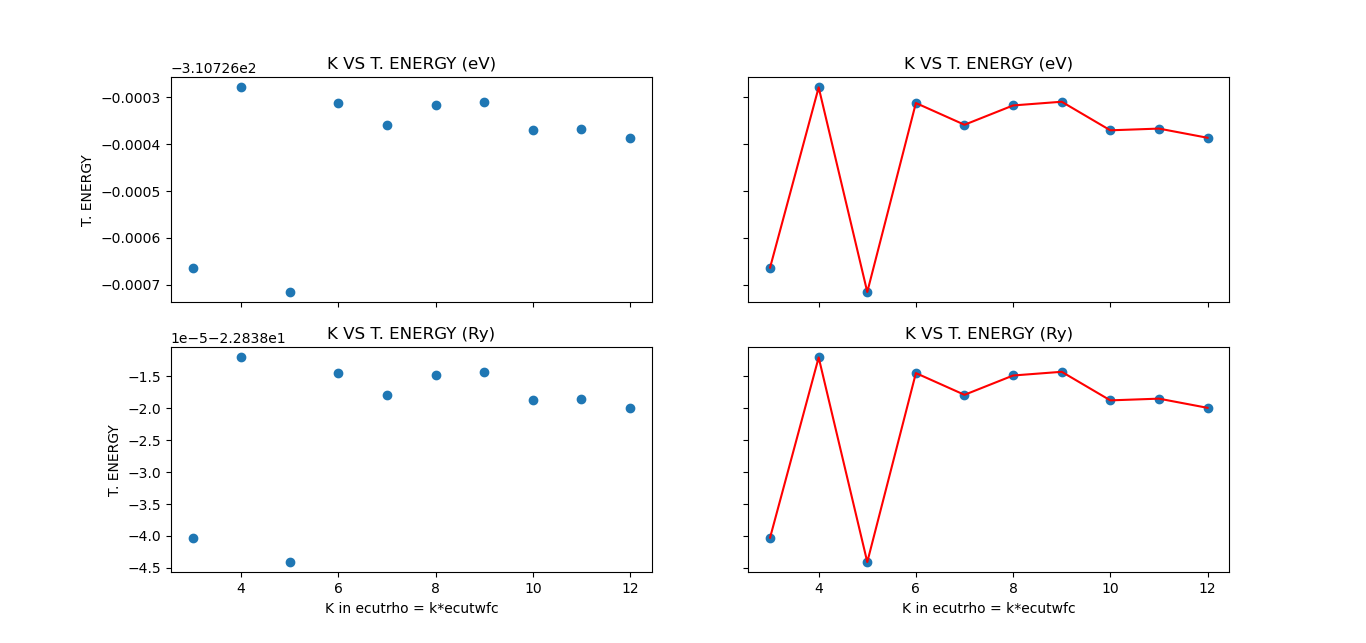
\includegraphics[scale=0.52]{images/k_vs_T_energy.png}
    \caption{Gráfica que nos muestra la energía total del sistema contra la variación del parámetro k, nos centramos en el intervalo [4,12]}
\end{figure}

Observación: el valor de la variable dependiente (la energía total) empieza su convergencia cuando 
la variable independiente (ecutwfc) empieza a tomar valores cercanos a 8.

\newpage

\subsection{Optimización K-points [Silicio] }

La siguiente de las optimizaciones para el silicio será la de puntos K. En nuestro archivo input estos
tienen la forma de la siguiente expresión: $ i \; i \; i \; 0 \; 0 \; 0$ donde $ i \in \mathbb{N}  $ .

\vspace{0.5cm}

Buscamos obtener un valor mínimo para i de tal manera que podamos observar una convergencia en la 
energía del sistema.

\begin{figure}[H]
    \centering
    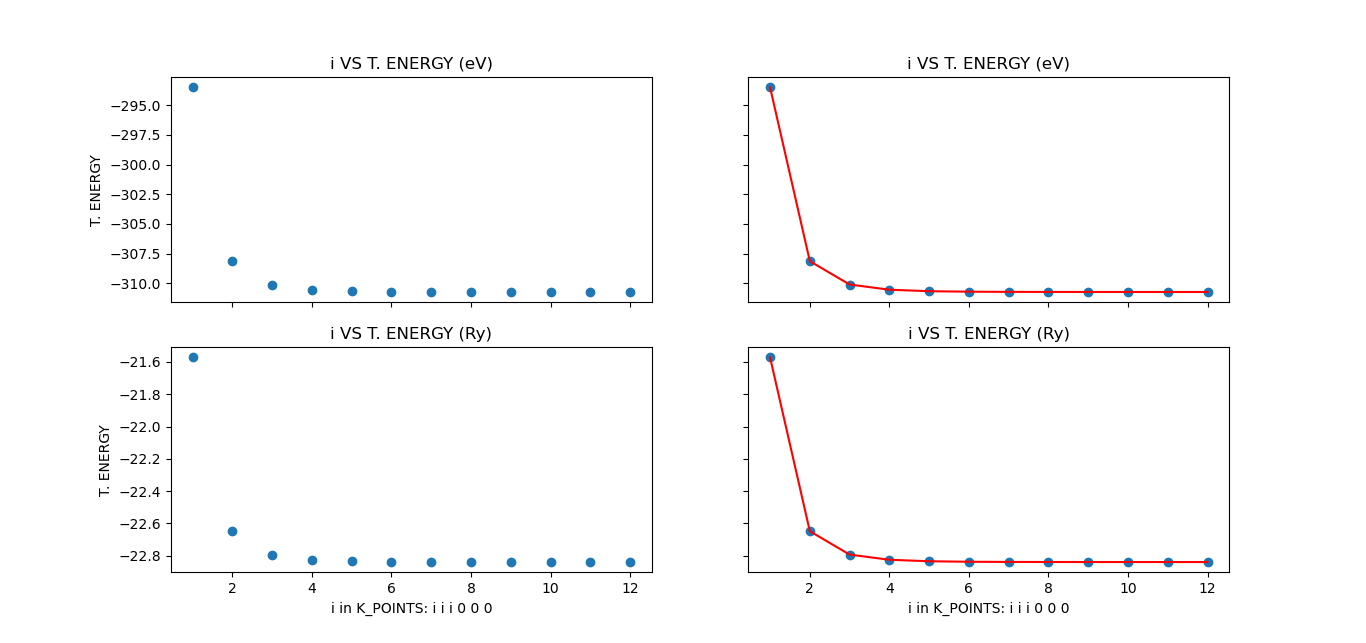
\includegraphics[scale=0.46]{images/k_points_vs_T_energy.png}
    \caption{Gráfica que nos muestra la energía total del sistema contra la variación del parámetro k, nos centramos en el intervalo [1,12]}
\end{figure}

Vamos a realizar la misma gráfica en un rectangulo de inspección más pequeño.

\begin{figure}[H]
    \centering
    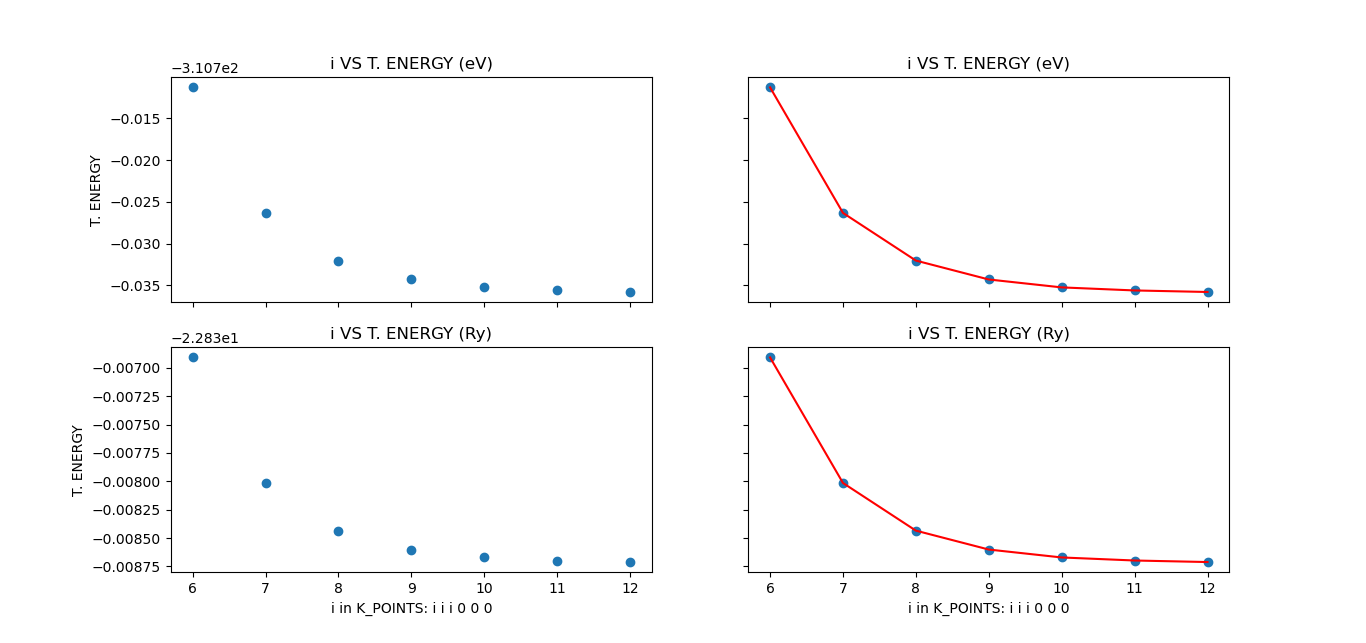
\includegraphics[scale=0.46]{images/k_points_vs_T_energy_neighborhood.png}
    \caption{Gráfica que nos muestra la energía total del sistema contra la variación del parámetro k, nos centramos en el intervalo [4,12]}
\end{figure}

Observación: el valor de la variable dependiente (la energía total) empieza su convergencia cuando 
la variable independiente (i) empieza a tomar valores cercanos a 8.


\subsection{Optimización Lattice parameter [Silicio] }

Ahora vamos a buscar optimizar el valor del paramétro de red, haremos una inspección probando valores
en el siguiente intervalo [4.4, 6.4].

\vspace{0.5cm}

Buscamos obtener un valor mínimo para el paramétro de red de tal manera que podamos observar una convergencia 
en la energía del sistema.

\vspace{0.5cm}

Empezaremos desde el 4.4 y para cada uno haremos un calculo del tipo "relax", repetiremos el proceso
en saltos de 0.1 en 0.1 hasta alcanzar el valor de 6.4.

\begin{figure}[H]
    \centering
    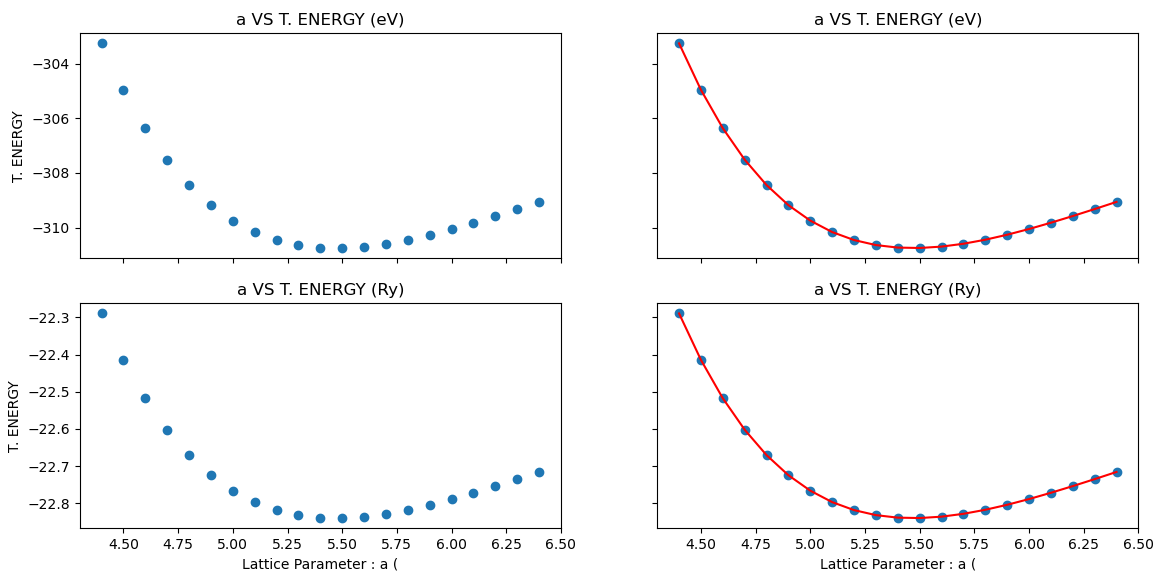
\includegraphics[scale=0.52]{images/lattice_parameter_vs_T_energy.png}
    \caption{Gráfica que nos muestra la energía total del sistema contra la variación del parámetro k, nos centramos en el intervalo [4.4,6.4]}
\end{figure}

Observación: el valor de la variable dependiente (la energía total) empieza su convergencia cuando 
la variable independiente (paramétro de red) empieza a tomar valores cercanos a 5.5.

\newpage

\subsection{Conclusiones [Silicio]}

Los resultados de la optimización del silicio nos llevan a elegir los siguientes valores como aquellos
óptimos luego de hacer los cálculos, los gráficos y el analísis de cada optimización.

\begin{table}[H]
    \begin{center}
        \begin{tabular}{| c | c |}
            \hline
            \multicolumn{2}{ |c| }{\textbf{Parámetros optimizados}} \\ \hline
            Ecutwfc & 30 \\ \hline
            K en Ecutrho & 8 \\ \hline
            i & 8 \\ \hline
            Parámetro de red & 5.5 \\ \hline
        \end{tabular}
        \caption{Valores elegidos después de cada optimización.}
        \label{tab: Parametros del Silicio optimizados}
    \end{center}
\end{table}

\newpage